%One of the main goals in scientific research is coming up to quantum simulation; this is due to the fact that in several physical fields there are mechanisms that cannot be simulated by classical computers: the essential aim is using a controlled quantum device to investigate another quantum system. Experiments have shown that superconducting circuits are able to manipulate and measure at the level of a few qubits and microwave photons, as a quantum simulator~\cite{Nat.Phys2012}. They can be treated as open systems because of the loss of photons, coupled to the feeding in additional photons through continuous external driving. Moreover, they are greatly flexible, because of their nanofabricated nature and almost every parameter involved is widely tunable. In~\cite{PhysRevX.7.011016}, it has been demonstrated that QED cavity lattices act as a controllable platform guiding understanding of non-equilibrium physics. 

\chapter{Open Many-Body Quantum Systems Coupled to External Baths}


\section{Basics of Dynamics}
As expressed in the previous chapter, an open quantum system can be described in terms of $\rho_S$, the reduced matrix given by averaging over the environment: 
\begin{equation}
    \rho_S = \Tr_E(\rho).
\end{equation}
Under certain conditions discussed in section~\ref{appr_dynam_oqs}, the evolution of $\rho_S$ is delineated by the Lindblad master equation:
\begin{equation}
\label{eqn:lindbladME_manyBody}
    \dot{\rho_S} = -i[H_{sys}, \rho_S] - \sum_{a=1}^{N^2-1} \gamma_a\mathcal{D}[L_a]\rho_S,
\end{equation}
where the first term expresses the usual unitary evolution under the system Hamiltonian $H_sys$ and the second term represents the influence of the environment over the system through the dissipation rate $\gamma_a$ and the dissipators
\begin{equation*}
    \mathcal{D}[L_a]\rho_S \equiv \frac{1}{2} \Bigl( [L_a\rho_S, L_a^{\dagger}] + [L_a, \rho_S L_a^{\dagger}] \Bigl).
\end{equation*}
The Linblad operators determine the nature of the decoherence process, e.g. photon loss ($a$), qubit relaxation ($\sigma^-$), qubit dephasing ($\sigma^z$), and so on.
The steady-state solution can be found rewriting this equation in terms of a linear algebra problem. First of all, the Hilbert space for a system consisting of N spins, has an orthonormal Fock-state basis such as $\ket{\phi_1, \phi_2, \dots \phi_N}$.
For solving the equation
\begin{equation*}
    \dot{\rho}_S = 0,
\end{equation*}
outlining a \emph{superoperator formalism}~\cite{davRoss_wordpress} is advantageous. 
Every linear operator $\hat{A}$ acting on the Hilbert space $\mathcal{H}$ can be associated with a vector in a superoperator space:
\begin{equation*}
    \hat{A} = \sum_{ij} A_{ij} \ket{i}\bra{j} \quad \rightarrow \quad |A\rangle\rangle = \sum_{ij} A_{ij} \ket{i}\ket{j}.
\end{equation*}
This way, the density operator can be vectorized and re-arranged as a \emph{super-ket} $|\rho_S\rangle\rangle$ with $N^2$ components. So, the eq.~\ref{eqn:lindbladME_manyBody} can be formally rewritten in terms of the Liouvillian superoperator; the steady-state equation can be read as an eigenvalue equation:
\begin{equation}
\label{eqn:SS_masterEq}
    \hat{L}|\rho_S\rangle\rangle = 0.
\end{equation}
Its solution can be obtained computing the eigenvector of the $N^2 \times N^2$ super-operator $\hat{L}$ corresponding to the null eigenvalue.

It is important to stress the enormous size of the matrix even for rather small systems sizes. So, straightforward brute-force integration methods become useless because the complexity of the problem becomes quickly unmanageable.

\section{Quantum Simulators: Controllable Many-Body Systems}
In order to overcome the mentioned problem, over the years several analytical and numerical methods have been developed. In addition to these more "traditional" approaches, in the last years the idea of studying a quantum system by using another quantum system arose. The essential aim of this new strategy lies in the employment of controlled quantum devices called \emph{quantum simulators}; they are systems able to experimentally emulate the Hamiltonian model bearing the non-trivial properties of the system under study. The usefulness of this approach is twofold~\cite{Tomadin_Fazio}:  not only it allows to explore properties of the model in regions that are elusive to the analytical and numerical studies, but also it consents to test to which limits the Hamiltonian model is appropriate to describe the system or whether additional ingredients are required.

Since the Josephson junction arrays, that were probably the first quantum simulators in Physics History, much progress have been made especially with the advent of cold atoms in optical lattices.

\subsection{Cold Atoms in Optical Lattice}
The employment of cold atoms in optical lattices has proved to be a successful way to create simulators of a large variety of strongly interacting systems~\cite{ultracoldAtoms_condMatter}. 

An interesting study over the possibility of using cold atoms to simulate dissipative many-body systems, has been done by~\cite{BEC_dissipativeMBsimulator}. In this work, they discuss the example of a driven dissipative Bose-Einstein condensate of bosons, where atoms in optical lattice are coupled to a bath of Bogoliubov excitations; the atomic current represents local dissipation. It has been assumed that the atoms can be described by the Hubbard model, having the following Hamiltonian:
\begin{equation}
    \mathcal{H} = \mathcal{H}_0 + V \equiv -J \sum_{\langle i,j \rangle} a_i^{\dagger} a_j + \frac{1}{2}U \sum_i a_i^{\dagger 2} a_j^2,
\end{equation}
where $\mathcal{H}_0$ represents the kinetic energy of bosons hopping between
adjacent lattice sites with amplitude J, V is the onsite interaction
with strength U and $a_i$ ($a_i^{\dagger}$) are bosonic destruction (creation)
operators for atoms at i-th site. At this point, an appropriate choice of jump operators allows to couple the system to a bath so that it is driven to a pure many-body state by quasi-local dissipation. Applying standard linearization schemes in the weakly interacting situations led to obtain the solution of the master equation~\ref{eqn:SS_masterEq}. The steady-state solution seems to have properties similar to those of bosons in thermal contact to a heat bath.

\subsection{QED-Cavity Arrays}
In the last few decades the field of quantum simulators has been enriched by a new idea, based on arrays of QED cavities~\cite{Tomadin_Fazio} (sketched in fig.~\ref{fig:QED_cavities}), in which light resonates and interacts with matter contained therein.  A compelling aspect of this kind of devices is the competition between two phenomena: while on the one hand light-matter interaction inside the cavity leads to photon blockade, on the other photon hopping between neighbouring cavities favors delocalization.

QED cavities are mathematically described by the Jaynes-Cummings model~\cite{shore_knight}, in which one mode of the cavity interacts with a two-level system. Before we see how it is done, let us ignore for a moment the interaction light-matter. A single cavity confines several modes of electromagnetic field and each of them is quantized as a harmonic oscillator. If one considers a cavity with a single mode with frequency $\omega$, the Hamiltonian describing such a system can be written as
\begin{equation}
\label{eqn:single_cavity}
    \mathcal{H} = \omega a^{\dagger}_la_l,
\end{equation}
where $a_l (a_l^{\dagger})$ annihilates (creates) a quantum of light in the mode of the l-th cavity.
An array of cavities sufficiently close to allow for photon hopping, can be described by eq.~\ref{eqn:single_cavity} to which the following term should be added:
\begin{equation*}
    \mathcal{H}_{hop} = -J (a^{\dagger}_la_l + h.c.),
\end{equation*}
where J is associated with the tunneling rate.
Now, if the light-matter interaction is introduced, the Hamiltonian can be written in this way:
\begin{equation}
    \mathcal{H} = \sum_l \mathcal{H}_l^{(0)} - J \sum_{\langle l, l' \rangle}(a^{\dagger}_la_l + h.c.),
\end{equation}
where the term $\mathcal{H}_l^{(0)}$ describes the light-matter interaction. In particular, we want to study QED cavities so the Hamiltonian term $\mathcal{H}_l^{(0)}$ is the Jaynes-Cummings model:
\begin{equation}
\label{eqn:Jaynes-Cummings}
    \mathcal{H}_{l,JC}^{(0)} = \varepsilon \sigma^z_l + \omega a^{\dagger}_la_l + g(\sigma^+_l a_l + \sigma^-_l a_l^{\dagger}),
\end{equation}
where $\sigma^\pm_l$ are the raising/lowering operators for the two-level system and $\varepsilon$ states the transition energy between the two levels.
The spectrum of the Hamiltonian~\ref{eqn:Jaynes-Cummings} is anharmonic, meaning the presence of the two-level system induces a repulsion between the photons in the cavity, so that in the cavity can be present only a photon at the same time. Qualitatively, this can be explained by the fact that a single photon in the cavity modifies the effective resonance frequency, so that the injection of another photon is inhibited. This nonlinear process is known as \emph{photon blockade} and has been named in analogy of the Coulomb blockade effect of electron transport through mesoscopic devices.
% QED cavities
    % sketch of QED cavities
    % optical cavities: photon blockade effect
    % Jaynes-Cummings nonlinearities
% pag. 55 Carusotto-Ciuti
% fig.10 di Noh2016

\begin{figure}
    \centering
    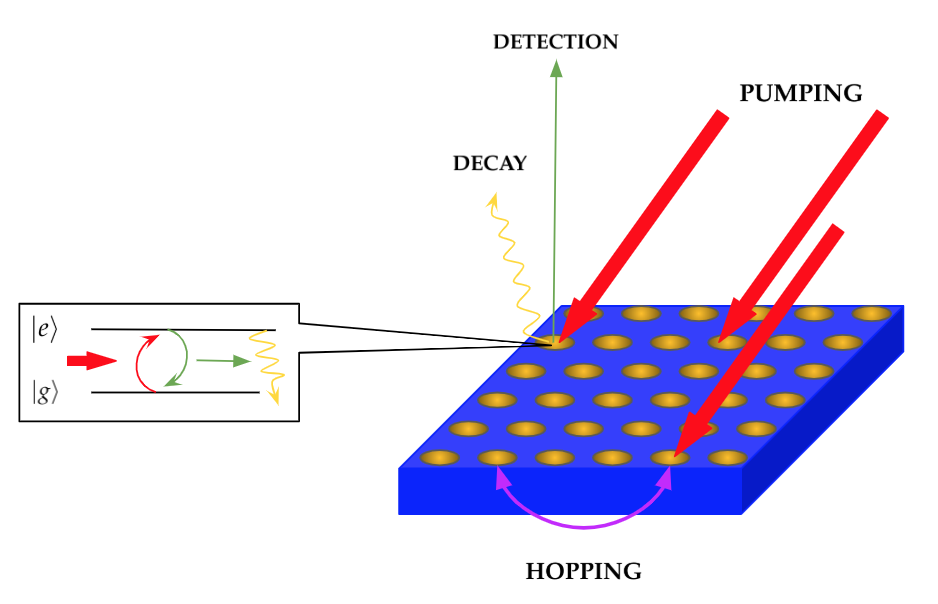
\includegraphics[scale=0.7]{Figures/QED_cavity.png}
    \caption{Sketch of array of QED cavities. In the inset there is a draft of the interaction between the two-level system and the photon resonating in the cavity and then decaying. Photons in the cavities have finite life-time, so there is a coherent external drive.}
    \label{fig:QED_cavities}
\end{figure}

% pag.5 Tomadin-Fazio per optical lattices vs cavity arrays

\subsection{Superconducting Circuits}
As for QED-cavities, also for superconducting circuits, or QED-circuits, is central light-matter interaction. In this simulators~\cite{supercircuitsQED}, the quantum "particles" are excitations, not physical particles subjected to conservation laws, so they naturally access non-equilibrium physics. Photonic mode can be realized with on-chip microwave resonators, typically Fabry-Perot kind of cavities. A qubit coupled to such a resonator can be described by the Jaynes-Cummings model:
\begin{equation}
    \mathcal{H}_{JC} = \omega_r a^{\dagger}a+ \varepsilon\sigma^+\sigma^- + g(a\sigma^+ + a^{\dagger}\sigma^-),
\end{equation}
where $\omega_r$ and $\varepsilon$ are the the photon and qubit excitation frequencies, and $a^{\dagger}$, a, $\sigma^+$ and $\sigma^-$ denote the corresponding raising and lowering operators.

Simulations of small spin chains are also possible by directly coupling a number of superconducting qubits49. In this experi- ment, a chain of eight ferromagnetically coupled spins in a one- dimensional chain was simulated with uniform coupling between nearest-neighbour spins. The ends of the chain were polarized in opposite directions, and an effective magnetic field gradient was in- duced by locally tuning each qubit transition energy,

\section{Quantum Simulation of Spin Systems}
Interacting two level systems, either spins or qubits, are of central importance in Quantum Information and Condensed Matter Physics. 
%\textcolor{red}{In magnetic compounds where spin lattices appear naturally the addressability of individual spins is unfortunately extremely hard to achieve because the spatial separation between neighboring spins is very small and the timescales of interesting processes can be very short.}

Since the discover of the \emph{photon blockade}~\cite{ph_blockade} arose the fact that the cavity mode is well described by a spin-$1/2$ Hamiltonian. Few years later, the Jaynes-Cummings model in the Mott regime was shown to simulate a XY spin model~\cite{angelakis}. In particular, the studied system consisted of coupled electromagnetic cavities doped with single two-level system; it is shown the possibility of observing an insulator phase of total (atomic plus photonic, i.e. \emph{polaritonic}) excitations. From such a system, an effective XY Hamiltonian arises, with spin up (down) corresponding to the presence (absence) of a polariton.

A scheme for realizing the Ising spin-spin interaction has been proposed in~\cite{LiGuGong}, where a system consisting in trapped two-level atoms in a one dimensional coupled microcavities. 

A more complicated system has been investigated in~\cite{Hartmann_XYZ}, which uses three-level atoms in micro-cavities coupled to each other via the exchange of virtual photons; it is shown that it can model an anisotropic Heisenberg spin-1/2 chain in an external magnetic field. The two spin polarizations $\ket{\uparrow}$ and $\ket{\downarrow}$ are represented by two long-lived atomic levels of a $\Lambda$ level-structure; let us see why. The quantized mode of the cavity together with external lasers can induce Raman transition between these two lowest-lying states.  With appropriately chosen detunings, the dominant Raman transition between the two lowest-lying states involves one laser and one cavity photon. This implies that the emission and absorption of virtual photons in the cavity is confined to only two states per atom, the long-lived ones, so that can be described by a spin-1/2 Hamiltonian. The coupling of virtual photons between neighbouring cavities simulates $\sigma^x\sigma^x$ and $\sigma^y\sigma^y$ interactions; the effective spin can be coupled to an effective magnetic field $\sigma^z$; using the same atomic level configuration but a different set-up of the external sources an effective $\sigma^z\sigma^z$ interaction is obtained.

It has been possible using superconducting circuits to simulate small spin chains, by directly coupling a number of superconducting qubits~\cite{8spinChain_simulatedByQubits}. Fig.\ref{fig:superconductinCircuit_SpinSystem} shows two superconducting loops in the qubit, each subject to an external flux bias $\Phi_{1x}$ and $\Phi_{2x}$. The dynamics of the device can be modelled as a quantum mechanical double-well potential. The two lowest energy states of the system correspond to clockwise or anticlockwise circulating current in loop 1. Considering only these two states (in the limit of low temperature it is a valid approximation), the qubit dynamics is that of an Ising spin. Qubits are then coupled together using programmable coupling elements; this allows to tune the spin coupling in a continous way between ferromagnetic and antiferromagnetic. The behaviour of this system is well described by an Ising model Hamiltonian:
\begin{equation*}
    \mathcal{H} = \sum_{i=1}^{N} h_i\sigma_i^z + \sum_{i,j=1}^{N} J_{ij}\sigma_i^z\sigma_j^z.
\end{equation*}
In this way, it has been possible to simulate a one-dimensional 8-sites spin chain, with the ends polarized in opposite directions.

\begin{figure}
    \centering
    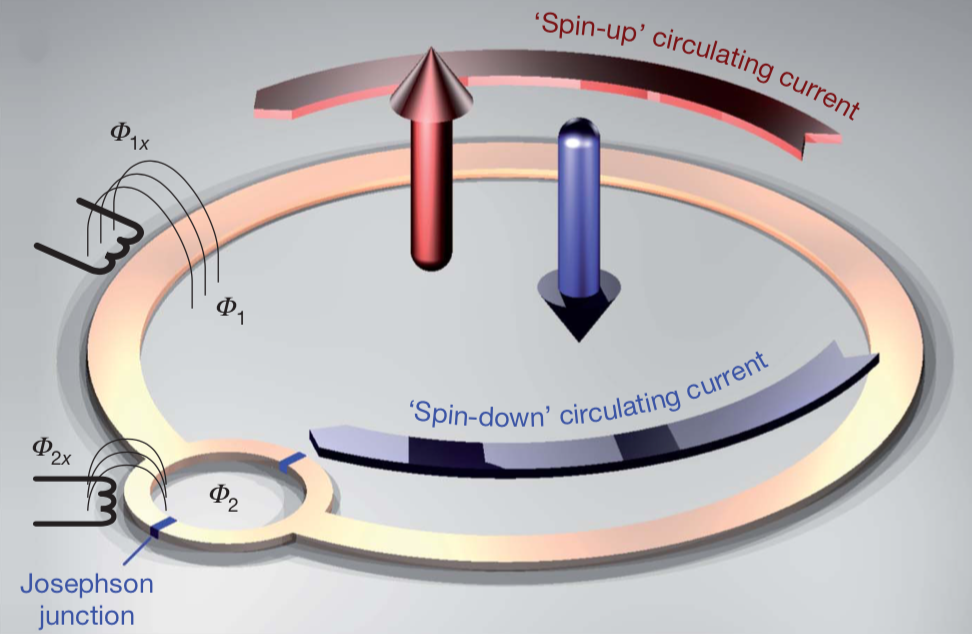
\includegraphics[scale=0.5]{Figures/superconductinCircuit_SpinSystem.png}
    \caption{Simplified schematic of a superconducting flux qubit \\acting as a quantum mechanical spin~\cite{8spinChain_simulatedByQubits}.}
    \label{fig:superconductinCircuit_SpinSystem}
\end{figure}